Relational databases consist of sets of tables designed to minimise data redundancy, possibly through the Normalisation process.  Data is therefore dispersed throughout those tables and, in order to solve a requirement, it will generally be necessary to bring together a number of fields from various related tables.  

\subsection{Cartesian Product}
This is the result of using more than one table in an unstructured way (Oracle cannot automatically interpret and use anything about relationships between tables).  What results would you expect to obtain with the following  instruction?



\begin{center}
\begin{minipage}{4.849cm}
   

\includegraphics[width=4.341cm,height=4.341cm]{images/img (36).png}
 

   

\includegraphics[width=1.582cm,height=0.674cm]{images/img (15).png}
 
\end{minipage}
\end{center}
D1\ \ SELECT ENAME, DNAME 

\ \ FROM EMP

\ \ CROSS JOIN DEPT ;

\begin{flushleft}
\tablefirsthead{}
\tablehead{}
\tabletail{}
\tablelasttail{}
\begin{supertabular}{|m{9.911cm}|}
\hline
Before you run this statement answer the first question.

How many rows would you expect?

Run the statement!

How many are displayed?

Does it look right?

Why not?

Where have the rows been generated from?\\\hline
\end{supertabular}
\end{flushleft}
If any column name occurs in more than one table, and that column is used anywhere in the query then it must be identified by specifying the table name (or alias) as a prefix.  If this is not done then an error message indicating that the column name is ambiguous will be returned. 

D2\ \ SELECT ENAME, DNAME, DEPTNO

\ \ FROM EMP

\ \ CROSS JOIN DEPT ;

\ \ Run this query. What error are you getting? Why?

\begin{center}
\begin{minipage}{14.605cm}
\end{minipage}
\end{center}
Most Database Management Systems now support the ANSI/ISO join syntax although some DBMSs, Oracle included, do continue to support their own non-standard formats.

\clearpage\subsection{Equi Joins}
These joins, also called SIMPLE JOINS, are the most common form and return rows from two joined tables based upon an equality condition in an ON clause.

\ \   SELECT\ \ column-list

\ \   FROM \ \ table\_name1 

\ \   INNER JOIN\ \ table\_name2 

\ \ \ \ ON \ \ join-condition

\ \ [ WHERE\ \ other criteria ]

In general the join condition will indicate that the columns should be equal:

\ \ SELECT \ \ ACCNO, NAME

\begin{center}
\begin{minipage}{4.692cm}
\begin{flushright}
\tablefirsthead{}
\tablehead{}
\tabletail{}
\tablelasttail{}
\begin{supertabular}{|m{2.4919999cm}|m{1.798cm}|}
\hline
ACCNO &
NAME\\\hline
1494315 &
J Doe\\\hline
1245890 &
J Doe\\\hline
5418490 &
R Best\\\hline
5418490 &
J Best\\
\end{supertabular}
\end{flushright}
\end{minipage}
\end{center}
\ \ FROM \ \ CUST  

\ \ INNER JOIN\ \ CUSTACC 

\ \ \ \ ON \ \ CUST.REFNO = CUSTACC.REFNO ;

D3\ \ Now repeat D1 but join the tables appropriately.



\begin{center}
\begin{minipage}{4.849cm}
   

\includegraphics[width=4.341cm,height=4.341cm]{images/img (37).png}
 

   

\includegraphics[width=1.582cm,height=0.674cm]{images/img (15).png}
 
\end{minipage}
\end{center}
\begin{flushleft}
\tablefirsthead{}
\tablehead{}
\tabletail{}
\tablelasttail{}
\begin{supertabular}{|m{11.329cm}|}
\hline
Select

From

INNER Join

On\\\hline
\end{supertabular}
\end{flushleft}
D4\ \ Display each employee's name along with the city they work in.

\begin{flushleft}
\tablefirsthead{}
\tablehead{}
\tabletail{}
\tablelasttail{}
\begin{supertabular}{|m{11.361cm}|}
\hline
Select

From

INNER Join

On

\\\hline
\end{supertabular}
\end{flushleft}


\begin{center}
  

\includegraphics[width=1.06cm,height=0.903cm]{images/img (2).png}

\end{center}
Have you noticed that the join condition (after ON) always occurs on the same columns? The next question uses that property.

D5\ \ Draw an Entity Relationship diagram of the two tables used in D3 and D4. Show the relationship between these two tables and the primary and foreign keys used.

\begin{flushleft}
\tablefirsthead{}
\tablehead{}
\tabletail{}
\tablelasttail{}
\begin{supertabular}{|l|}
\hline
\\\hline
\end{supertabular}
\end{flushleft}
D6\ \ Display the name of each department and the names of the staff who work in each of them.

\begin{flushleft}
\tablefirsthead{}
\tablehead{}
\tabletail{}
\tablelasttail{}
\begin{supertabular}{|m{14.303cm}|}
\hline
Select

From

INNER Join

On\\\hline
\end{supertabular}
\end{flushleft}
D7  \ \ Find the name (not the number!) and salary of employees in DALLAS.



\begin{center}
  
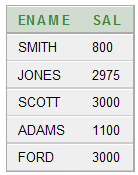
\includegraphics[width=3.669cm,height=4.586cm]{images/img (38).png}

\end{center}
\begin{flushleft}
\tablefirsthead{}
\tablehead{}
\tabletail{}
\tablelasttail{}
\begin{supertabular}{|m{11.110001cm}|}
\hline
Select

From

INNER JOIN

ON

Where\\\hline
\end{supertabular}
\end{flushleft}
D8\ \ Display details of employees in ACCOUNTING.  (Don't answer this by using  {}'WHERE Deptno = 10'.  Use two tables to find the department by name).

\begin{flushleft}
\tablefirsthead{}
\tablehead{}
\tabletail{}
\tablelasttail{}
\begin{supertabular}{|m{14.793cm}|}
\hline
Select

\\\hline
\end{supertabular}
\end{flushleft}
D9\ \ Display the department name along with the lowest and highest salaries in each department.

\begin{flushleft}
\tablefirsthead{}
\tablehead{}
\tabletail{}
\tablelasttail{}
\begin{supertabular}{|m{14.583cm}|}
\hline
Select

\\\hline
\end{supertabular}
\end{flushleft}
D10\ \ What are the highest and lowest incomes (including commission) in the Sales department?  (You might like to refer back to exercise C8.)

\begin{flushleft}
\tablefirsthead{}
\tablehead{}
\tabletail{}
\tablelasttail{}
\begin{supertabular}{|m{14.583cm}|}
\hline
Select

\\\hline
\end{supertabular}
\end{flushleft}
D11\ \ Display the department name and number of employees in departments with 5 or more employees.  (Refer back to C16.)

\begin{flushleft}
\tablefirsthead{}
\tablehead{}
\tabletail{}
\tablelasttail{}
\begin{supertabular}{|m{10.648cm}|}
\hline
Select

From

INNER Join

\begin{center}
\begin{minipage}{4.849cm}
   

\includegraphics[width=4.341cm,height=4.341cm]{images/img (39).png}
 

\centering\arraybslash 

\includegraphics[width=1.582cm,height=0.674cm]{images/img (15).png}
 \end{minipage}
\end{center}
On

Group By

Having\\\hline
\end{supertabular}
\end{flushleft}
D12\ \ Find out the total income for all employees in each city.  This will include commission.

\begin{flushleft}
\tablefirsthead{}
\tablehead{}
\tabletail{}
\tablelasttail{}
\begin{supertabular}{|m{14.352cm}|}
\hline
Select

From

INNER Join

On 

GROUP BY\\\hline
\end{supertabular}
\end{flushleft}
In many cases there will be more than two tables involved.  If there are n tables involved in the instruction, then there are (n-1) table relationships to be defined using JOIN and ON.

 \ \ SELECT \ \ CUST.REFNO, NAME, ACC.ACCNO, BALANCE

\ \ FROM \ \ CUST  

\ \ \ \ INNER JOIN\ \ CUSTACC 

\ \ \ \ \ \ ON \ \ CUST.REFNO = CUSTACC.REFNO

\ \ \ \ INNER JOIN\ \ ACC 

\ \ \ \ \ \ ON \ \ CUSTACC.ACCNO = ACC.ACCNO ;



\begin{center}
\begin{minipage}{10.075cm}
\begin{flushleft}
\tablefirsthead{}
\tablehead{}
\tabletail{}
\tablelasttail{}
\begin{supertabular}{|m{1.742cm}|m{2.55cm}|m{2.552cm}|m{2.43cm}|}
\hline
REFNO &
NAME &
ACCNO &
BALANCE\\\hline
A123 &
J Doe &
1494315 &
.5\\\hline
A123 &
J Doe &
1245890 &
234.5\\\hline
B127 &
R Best &
5418490 &
1789.4\\\hline
B127 &
J Best &
5418490 &
1789.4\\
\end{supertabular}
\end{flushleft}
\end{minipage}
\end{center}
Non-Equi Join

Most ON clauses will use = for the relationship, but other options are possible ({\textless}, {\textgreater})

For example, table EMP contains details of Employees.  One piece of data is their Salary.  The SALGRADE table holds the Grade and the salary range (stated as the low and high values) applicable to that grade.  How do we find the Grade that any employee is on?  We cannot do this directly as the SALGRADE table does not contain a list of all possible salaries.  But we can identify the grade by selecting the row where the employee's salary is BETWEEN LOSAL and HISAL (assuming the grades do not overlap).

D13  \ \ Produce a list that will show the salary grade each employee is on.  Display the name, job, salary and grade with the output in ascending order of salary, and with those on the same salary ordered alphabetically.

\begin{flushleft}
\tablefirsthead{}
\tablehead{}
\tabletail{}
\tablelasttail{}
\begin{supertabular}{|m{14.793cm}|}
\hline
Select

From

INNER Join

On

Order By\\\hline
\end{supertabular}
\end{flushleft}
D14\ \ Display employee name, job, salary and department name for those people on grade 3.



\begin{center}
  
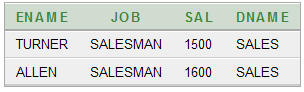
\includegraphics[width=6.897cm,height=2.081cm]{images/img (40).png}

\end{center}
\begin{flushleft}
\tablefirsthead{}
\tablehead{}
\tabletail{}
\tablelasttail{}
\begin{supertabular}{|m{8.332cm}|}
\hline
Select

From

INNER JOIN

ON

INNER JOIN

ON

WHERE\\\hline
\end{supertabular}
\end{flushleft}

This page is intentionally blank.